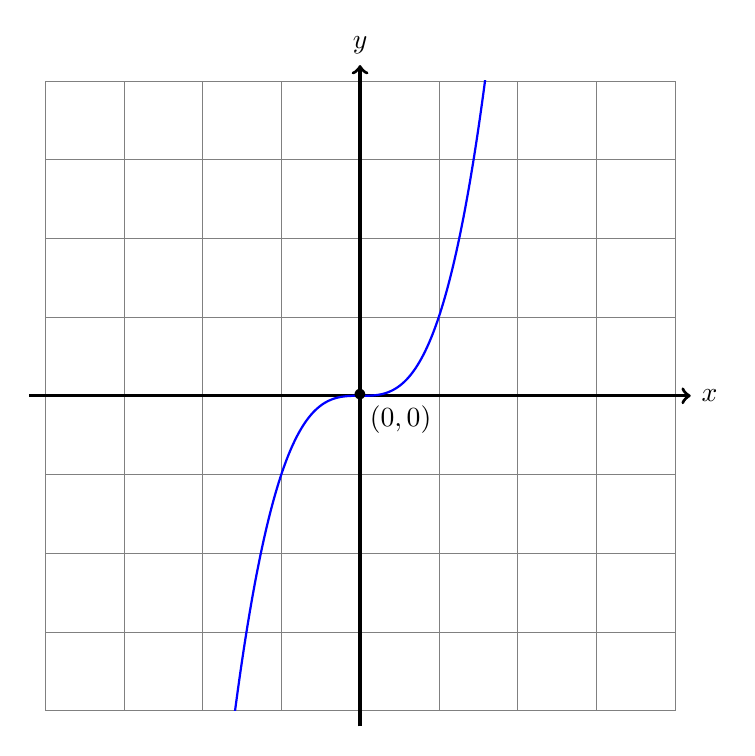
\begin{tikzpicture}
  \draw[very thin,color=gray] (-4,-4) grid (4,4);

  \draw[very thick,->] (-4.2,0) -- (4.2,0) node[right] {$x$};
  \draw[very thick,->] (0,-4.2) -- (0,4.2) node[above] {$y$};

  \begin{scope}
    \clip (-4,-4) rectangle (4,4);
    \draw [color=blue,thick] plot[smooth,samples=500,domain=-4:4] (\x,{(\x)^3});
  \end{scope}

  \node at (0,0) {$\bullet$};
  \node [below right] at (0,0) {$(0,0)$};
\end{tikzpicture}
